\section{Daten}


\subsection{Daten Auswahl}
Es gibt keine frei zugänglichen umfassenden Datasets für Sprachidentifikations-Aufgaben. Datensets wie das \textit{NIST Language Recognition Evaluation}\cite{nist} sind nur unter teuren Gebühren zugänglich. Wie verwandte Arbeiten empfehlen \cite{iLID}, wird darum ein eigenes Datenset zusammengestellt. Es werden gleichmässig Daten zu den Sprachen Deutsch, Englisch, und Französisch gesammelt. Die Daten stammen einerseits vom \textit{Voxforge}\cite{voxforge} Datenset und von \textit{Youtube}\cite{youtube}.

\paragraph{Voxforge} ist ein open-source Datenset für die Spracherkennung. Es besteht aus vielen kurzen (1-10s), von Benutzern hochgeladenen, Audiodateien. Die englische Sprache dominiert mit rund 120h Audio das Datenset. Über alle drei Sprachen verteilt sind es 190h. Die Audioqualität variiert je nach Benutzer.

Die Sprache ist langsam und deutlich verständlich. Sie hört sich eher künstlich an, im Vergleich zu einem natürlichem Gespräch.

\paragraph{Youtube}dient als Quelle für natürlichere Sprache. Es werden angesehene Nachrichtenkanäle wie CNN, ARD, etc. verwendet. Die Sendungen haben den Vorteil, dass oft fremde Gäste eingeladen werden, was zu einer grossen Variation der Sprecher führt. Ausserdem kommen oft natürliche Hintergrundgeräusche dazu. Zum Schluss ist die Datenmenge die hier erhältlich ist, praktisch unbeschränkt gross.

\begin{table}[h]
    \begin{subtable}[t ]{0.45\textwidth}
        \centering
        \begin{tabular}[t]{l || c c}
        Sprache & Voxforge & Youtube \\
        \hline \hline
        Französisch & 20h & 50h\\
        Deutsch & 22h & 60h\\
        Englisch & 23h & 200h\\
        \end{tabular}
        \caption{Verteilung der Datenmenge}
        \label{tab:amount}
    \end{subtable}
    \hfill
    \begin{subtable}[t ]{0.45\textwidth}
        \centering
        \begin{tabular}[t]{l || l}
        Sprache & Kanäle \\
        \hline \hline
        Französisch & France24, FranceInfo\\
        Deutsch & ARD, ZDF\\
        Englisch & CNN,  BBC
        \end{tabular}
        \caption{Youtube Kanäle}
        \label{tab:channels}
    \end{subtable}
    \caption{Daten Auswahl}
    \label{tab:data}
\end{table}


\subsection{Daten Splitt}
Zu grosse Datenmengen sind für das Training problematisch. Sie sind technisch aufwendig und sehr langsam in der Verarbeitung. Zudem ist es immer das Ziel eines Algorithmus, mit möglichst wenigen Daten auszukommen. Darum wird das Datenset auf 100'000 Stücke reduziert, was ungefähr 139h insgesamt ausmacht. Die Daten stammen zufällig zu gleichen Teilen sowohl aus Youtube wie von Voxforge. Die einzelnen Sprachen sind gleichgewichtig repräsentiert.

Das Datenset wird wiederum in \textit{Trainingset}, \textit{Validationset}, und \textit{Testset} aufgeteilt zu den Anteilen 80\%, 10\% und 10\%. Das \textit{Trainingset} wird, wie der Name preisgibt, für das Training verwendet. Das \textit{Validationset} wird verwendet um zu beobachten, wie das Modell auf neue Daten reagiert. Die \textit{Hyperparamter} (Parameter die das Netzwerk nicht selber lernen kann, z.B die Anzahl Knoten) werden manuell so angepasst dass das Netzwerk möglichst gut auf dem \textit{Validationset} abschneidet. Zuletzt wird das \textit{Testset} in Betracht gezogen, um die Leistung auf gänzlich neue Daten zu erforschen.

\subsection{Preprocessing}
Sprache besteht aus Wörtern und Wörter sind grundsätzlich eine Abfolge von Lauten. Verschiedene Sprachen unterscheiden sich an den verschiedenen Abfolgen von Lauten, manchmal sogar an den verwendeten Lauten selbst. Die kleinste relevante Einheit für Spracherkennung, sowohl für den Menschen wie die Maschine, ist also ein Laut.

Wenn der Computer mit dem Mikrofon aufnimmt, misst er kleinste Druckunterschiede, bzw. Schallwellen. Eine unkomprimierte Audiodatei zeigt den Schalldruck über die Länge der Aufnahme, siehe Abbildung \ref{img:preprocessing} \textit{(oben)}.
Die einzelne Schallwelle ist für den Menschen nicht erkennbar, deshalb ist sie auch für die Sprache von keiner Bedeutung. Erst mehrere Schallwellen, bzw. die daraus folgende Frequenz lässt sich als Laut hören. [siehe KAMBOR]

Das Verfahren um aus einer Schallwelle die unterschiedlichen Frequenzen zu bestimmen heisst \textit{Fourier-Transformation} \cite{fourrier}. Das Neuronale Netz müsste dieses Verfahren erlernen um dann aus den Lauten die Sprache erkennen zu können. Allerdings ist die Fourrier Transformation sehr komplex und fordert den Computer darum viel. Um dem Algorithmus die Aufgabe zu erleichtern kann man ihm darum als Eingabe die berechneten Laute geben anstatt der rohen Schallwelle.

Die Prozedur dem Algorithmus bereits vorgerechnete Werte zu füttern, heisst \textit{Preprocessing} und ist weit verbreitet im Feld von \textit{Machine learning} Feld. Das vorrechnen ist unter dem Namen \textit{Feature engineering} bekannt. \textit{Features}, also Merkmale z.b Laute werden aus den Rohen Daten extrahiert. \parencite[vgl.][]{chollet}

\subsubsection{Spektrogramme}
\begin{figure}[hbt]
	\centering
		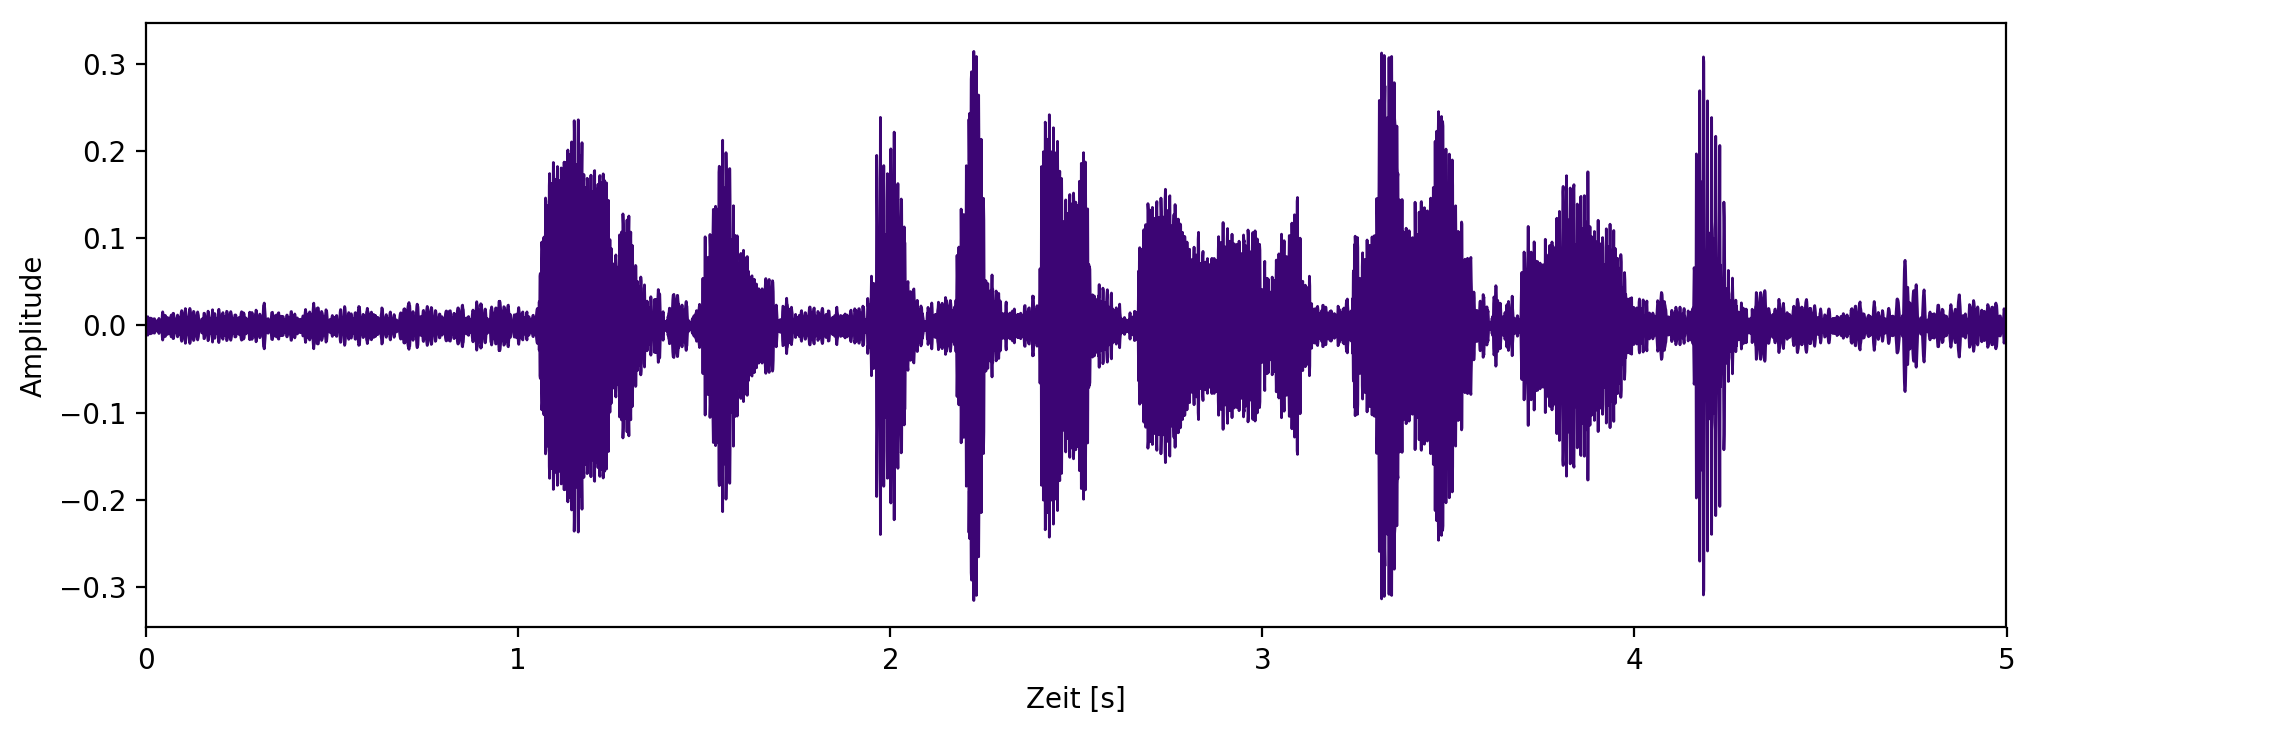
\includegraphics[width=0.6\textwidth]{assets/audio_raw.png}
		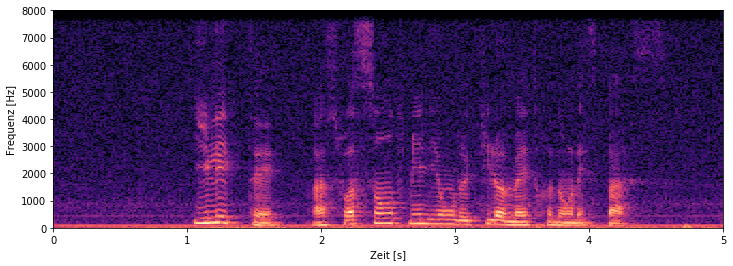
\includegraphics[width=0.6\textwidth]{assets/audio_log.png}
		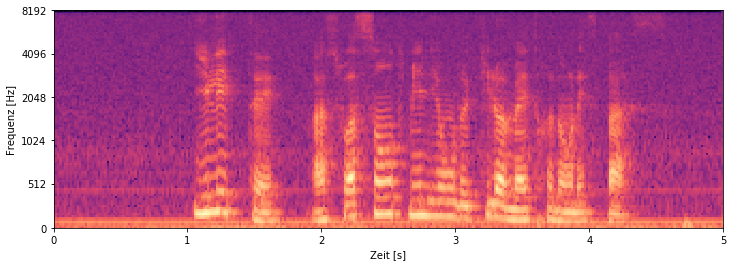
\includegraphics[width=0.6\textwidth]{assets/audio_mel.png}
	\centering
	\caption{Audio-Preprocessing: \textit{(oben)} Rohe Schallwelle, \textit{(mitte)}
		     Log-power Spectrogramm, 
		     \textit{(unten)} Mel Spectrogramm}
	\label{img:preprocessing}
\end{figure}

